\documentclass[10.5pt]{article}

\usepackage{amsmath}
\usepackage{textcomp}
\usepackage[top=0.8in, bottom=0.8in, left=0.8in, right=0.8in]{geometry}
% Add other packages here %
\usepackage{graphicx}
\usepackage{subcaption}
\usepackage{hyperref}
\usepackage{floatrow}
\usepackage[english]{babel}



% Put your group number and names in the author field %
\title{\bf Exercise 3\\ Implementing a deliberative Agent}
\author{Group \textnumero 9: Fengyu Cai, Wanhao Zhou}


% N.B.: The report should not be longer than 3 pages %


\begin{document}
\maketitle

\section{Model Description}

\subsection{Intermediate States}
% Describe the state representation %
For each vehicle, we define the state representation as follows, and the first three properties uniquely define a state.
\begin{enumerate}
	\item[-] \texttt{currentCity}. The city where the vehicle is currently in.
	\item[-] \texttt{taskOnBoard}. Tasks the vehicle has already undertaken.
	\item[-]	 \texttt{taskAvailable}. The remaining tasks to be undertaken (picked up).
	\item[-] \texttt{spaceLeft}. The remaining space for the vehicle to pick up tasks.
	\item[-]	 \texttt{cost}. I.e., $g(n)$, the cost paid so far (the distance travelled times the cost of the vehicle per km)
	\item[-] \texttt{heuristic}. I.e., $h(n)$, the estimated cost to the final state.
	\item[-] \texttt{totalCost}. I.e., $f(n)$, which equals to $g(n) + h(n)$.
\end{enumerate}

\subsection{Goal State}
% Describe the goal state %
The goal state is achieved if and only if there is no more \texttt{taskOnBoard} and no more \texttt{taskAvailable}. In our searching algorithm, we would consider this as the final state. Typically, in A*, when we reach the goal state, the algorithm will directly return the plan.

\subsection{Actions}
% Describe the possible actions/transitions in your model %
We run the algorithm directly on the states described above to search for an optimal state transition (from the initial state to the goal state) which yields the lowest cost. 

Between the neighbouring states, we can define the actions that lead from the previous state to the next state. Actions include:
\begin{enumerate}
	\item[-]\texttt{Move(nextCity)}. This action is chosen when two neighbouring states have different \texttt{currentCity}.
	\item[-]\texttt{Pickup(task)}. This is chosen when the \texttt{taskAvailable} fields are different, meaning that there are fewer tasks available, since one of them is already picked up. 
	\item[-]\texttt{Delivery(task)}. Similarly, this is chosen when the \texttt{taskOnBoard} fields are different.
	
\end{enumerate}

\section{Implementation}

\subsection{BFS}
% Details of the BFS implementation %
We implemented two versions of BFS algorithm, namely \texttt{BFS} and \texttt{BFS\_FAST}. The only difference is in the cycle detection part. BFS runs with the \texttt{Queue}. While the queue is not empty, the algorithm continues to run. When the first element of the queue is polled out, we would check if the state is final or not. If it is final we will record its final cost of the plan, and update the current best plan. The algorithm terminates when the queue is empty.

For the cycle detection, the slower BFS uses the technique similar as that of A*, meaning that we regard a state as redundant if there is already a copy in our \texttt{HashMap} and the current one has a cost greater than its previous copy. \texttt{BFS\_FAST} will not consider any states that have been visited, irrespective of the cost. Indeed, \texttt{BFS\_FAST} is the same as the algorithm given in the slides.

\subsection{A*}
% Details of the A* implementation %
A* runs with the heuristic function as an estimate of the cost till the final state. There are three major differences from BFS.
\begin{enumerate}
	\item[-] Instead of using the \texttt{Queue}, which polls element out in the order that is added, the algorithm uses \texttt{PriorityQueue} and set the key as the \texttt{totalCost}. \texttt{PriorityQueue} maintains a Min-Heap that each time we poll out the first element, it will be the state that has the lowest \texttt{totalCost}.
	\item[-] Like the slower version of BFS mentioned above, we maintain a \texttt{HashMap} that matches a state to its cost. We discard states that already have a copy in \texttt{HashMap} and the current one's cost is higher.
	\item[-] Once we poll out a goal state from the heap, the algorithm terminates and returns the plan.
\end{enumerate}

\subsection{Heuristic Function}
% Details of the heuristic functions: main idea, optimality, admissibility %
Let $T_A$ denotes all tasks available of the current state, and $T_B$ denotes all tasks already undertaken.
Our estimation heuristic of the current state $s$ is calculated via the following formula:
$$h(s) = \max_{t \in T_A\cup T_B} \mathrm{CostToGoal}(t)$$
CostToGoal is calculated separately for $T_A$ and $T_B$. If a task is not undertaken, we calculate the distance from current city to the pickup city plus the distance from the pickup city to delivery city, while for tasks on board, we only consider the distance from current city to the delivery city. The final distance times the cost per km gives the cost.

%Admissibility and optimality of $h(s)$.
We can easily verify that $h(s)$ underestimates the actual cost to the final state. From the triangle inequality we know that $h(s)$ equals to the actual cost if and only if all tasks' pickup city and delivery city are on the same line from the current city, and $h(s)$ will be lower otherwise. Since $h(s)$ underestimates the cost, this gives us admissibility and optimality of the heuristic function.


\section{Results}

\subsection{Experiment 1: BFS and A* Comparison}
% Compare the two algorithms in terms of: optimality, efficiency, limitations %
% Report the number of tasks for which you can build a plan in less than one minute %

\subsubsection{Setting}
% Describe the settings of your experiment: topology, task configuration, etc. %
We set the seed as $23456$. For different number of tasks, \texttt{BFS}, \texttt{BFS\_FAST} and \texttt{ASTAR} yields the same optimal plan (w.r.t the cost of the whole plan, i.e. the total traveling distance), given in Table~\ref{tab:my-table}. Also

\begin{figure}[h]
    \centering
    \begin{subfigure}{.3\textwidth}
        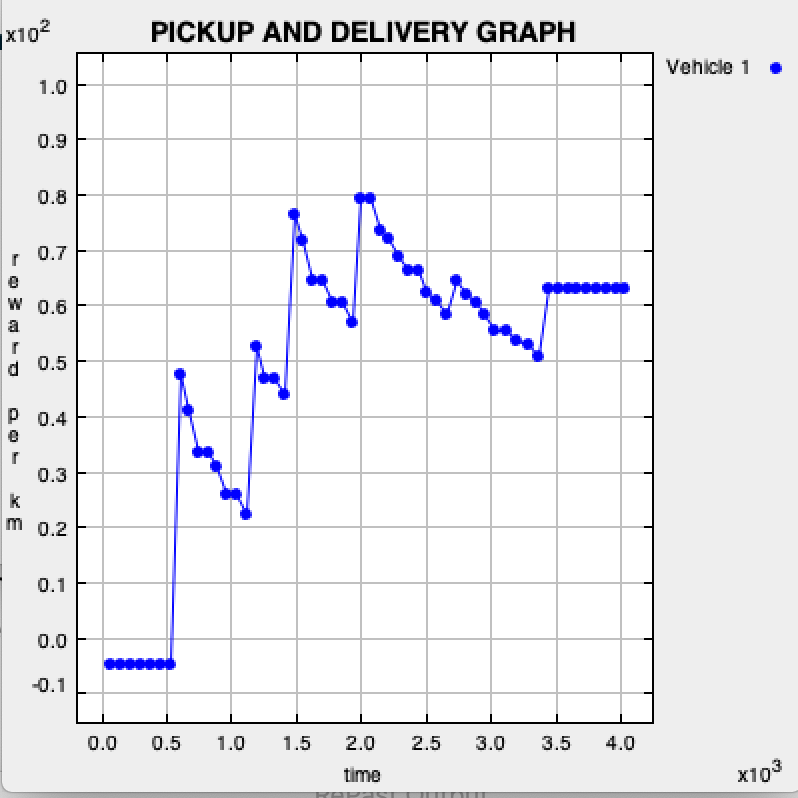
\includegraphics[width = \textwidth, height=4.5cm]{random-6task.png}
        \caption{Reward per km for random plan}
        \label{fig:growth-2-energy-100}
    \end{subfigure}%
    ~
    \begin{subfigure}{.3\textwidth}
        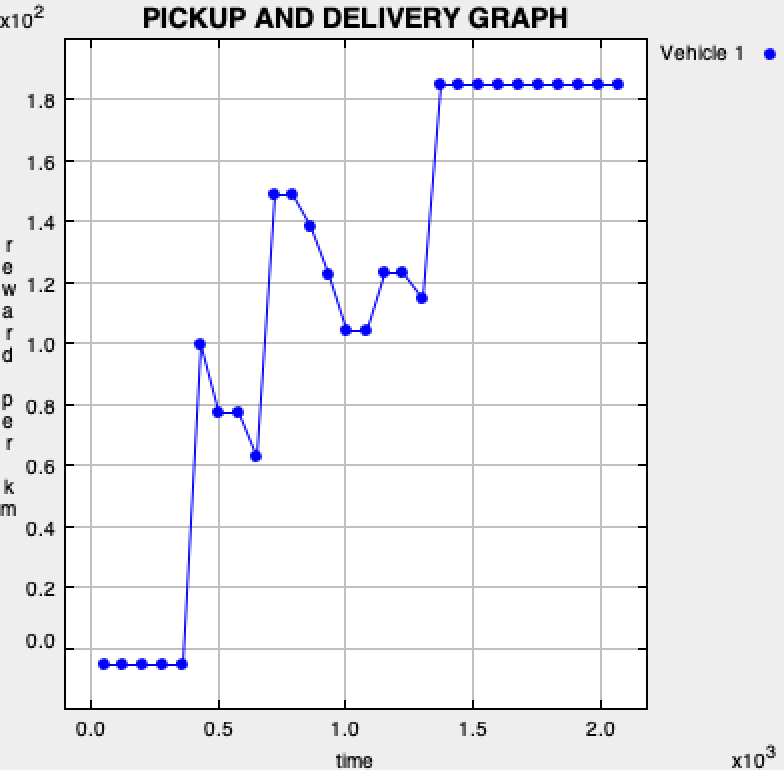
\includegraphics[width = \textwidth, height=4.5cm]{bfs-6task.png}
        \caption{Reward per km for BFS plan}
        \label{fig:energy-100-startEnergy-15-world-100-100}
    \end{subfigure}
    ~
    \begin{subfigure}{.3\textwidth}
        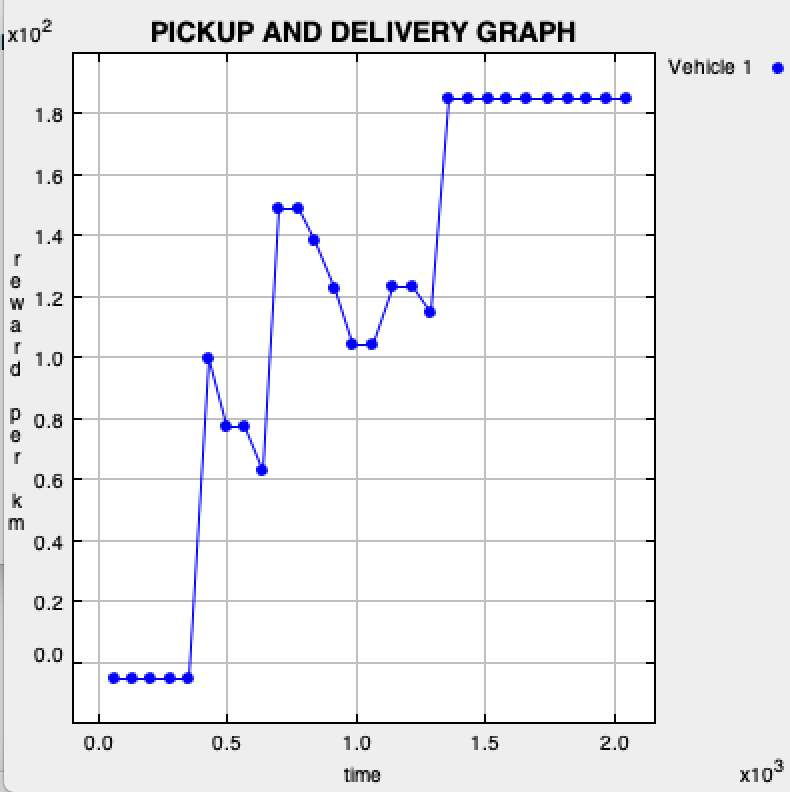
\includegraphics[width = \textwidth, height=4.5cm]{astar-6task.png}
        \caption{Reward per km for ASTAR plan}
    \end{subfigure}
    \caption{Experiment among different plan}\label{fig:exp-3}
\end{figure}

\begin{table}[!h]
\begin{center}
\begin{tabular}{|c|c|c|c|c|}
\hline
 \# Tasks	&\texttt{BFS}		&\texttt{BFS\_FAST}	&\texttt{ASTAR}		&Total Distance  \\ \hline
 6	&3.484s	&0.941s	&0.114s  &1380  \\ \hline
 7	&13.124s		&3.521s	&0.384s  &1610  \\ \hline
 8	&124.124s  &28.036s	&1.764s  &1710  \\ \hline
 9	&N/A  &N/A  &4.527s  &1720  \\ \hline
 10	&N/A  &N/A  &41.282s  &1820  \\ \hline
\end{tabular}
\caption{Runtime comparison of different algorithms}
\label{tab:my-table}
\end{center}
\end{table}

\subsubsection{Observations}
% Describe the experimental results and the conclusions you inferred from these results %
From Table 1, we could find out the plan generated by \texttt{BFS}, \texttt{BFS\_FAST}, and \texttt{ASTAR} are the same, and execution time increases exponentially for all of them. \texttt{ASTAR} is much faster than \texttt{BFS}. Also, from the Figure 1, both \texttt{BFS} and \texttt{ASTAR} greatly improve the delivery gain when the number of task is 6 compared with the naive plan.


\subsection{Experiment 2: Multi-agent Experiments}
% Observations in multi-agent experiments %

\subsubsection{Setting}
% Describe the settings of your experiment: topology, task configuration, etc. %
When the agent observe the change of the environment (pickup or delivery tasks in its plan), it will automatically re-generate the plan based on the current circumstance. Here, we set the total number of task is 8, and the default planning algorithm is \texttt{ASTAR}.

\begin{figure}[h]
    \centering
    \begin{subfigure}{.3\textwidth}
        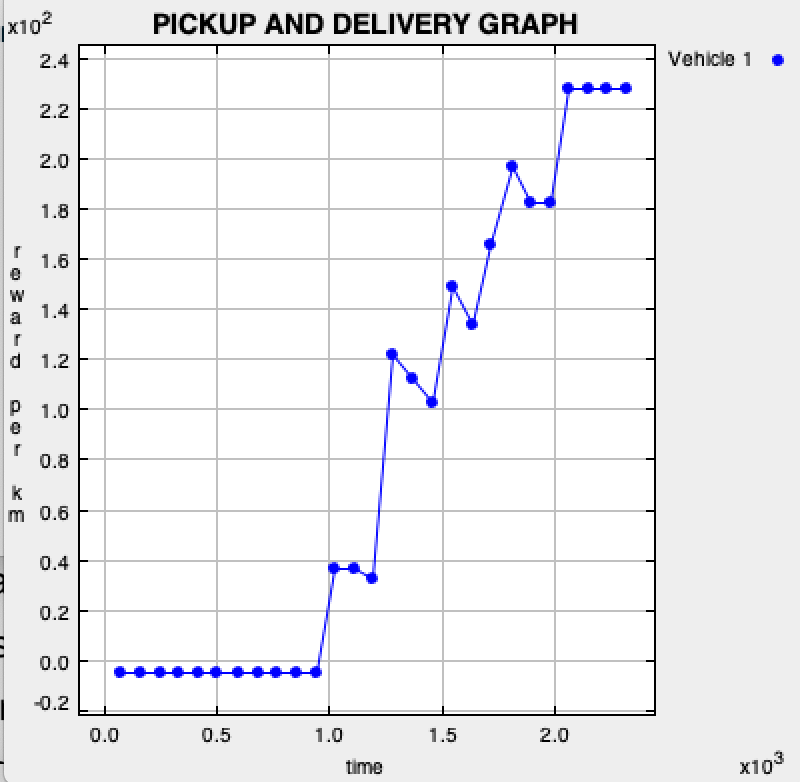
\includegraphics[width = \textwidth, height=4.5cm]{1agent-8task.png}
        \caption{Reward per km for agent-1}
        \label{fig:growth-2-energy-100}
    \end{subfigure}%
    ~
    \begin{subfigure}{.3\textwidth}
        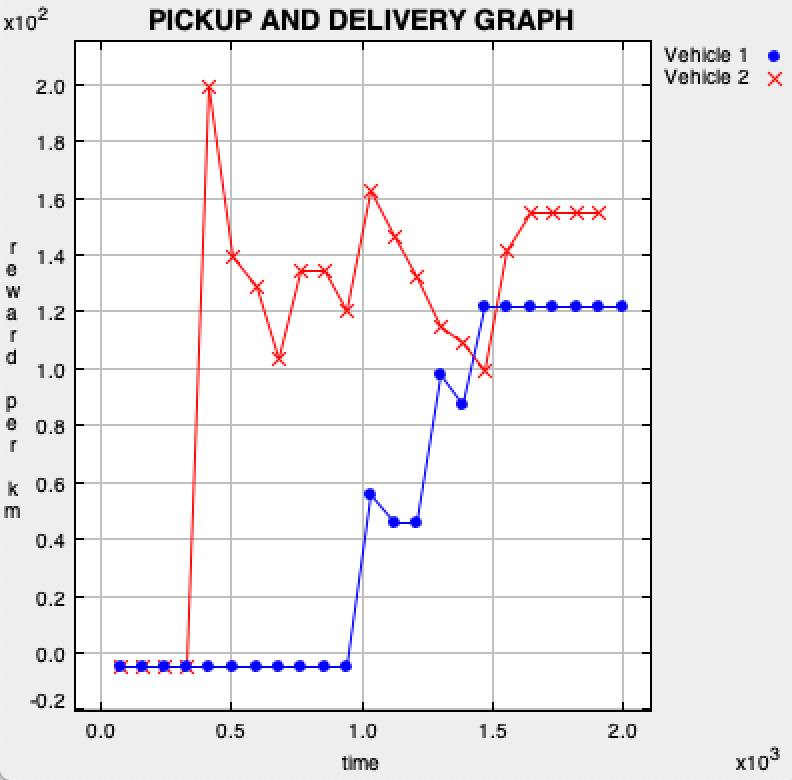
\includegraphics[width = \textwidth, height=4.5cm]{2agent-8task.png}
        \caption{Reward per km for agent-1 and agent-2}
        \label{fig:energy-100-startEnergy-15-world-100-100}
    \end{subfigure}
    ~
    \begin{subfigure}{.3\textwidth}
        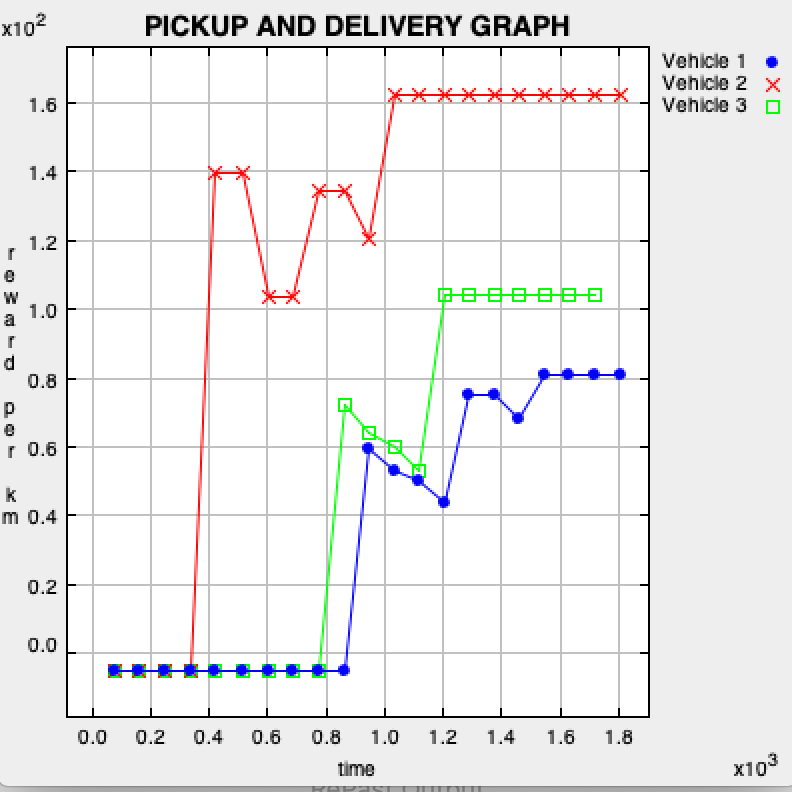
\includegraphics[width = \textwidth, height=4.5cm]{3agent-8task.png}
        \caption{Reward per km for agent-1, agent-2, and agent-3}
    \end{subfigure}
    \caption{Experiment for different number of agents}\label{fig:exp-3}
\end{figure}

\subsubsection{Observations}
% Describe the experimental results and the conclusions you inferred from these results %
From the experiments above, we find that with the increasing number of agents involved, the total time spent will be decreased, and the sum of gain per km will be higher.

\end{document}